% %******************************************************************************
% % % modos.tex %
% %******************************************************************************
% % % Title......: Modos de Operação % % Author.....: GSCAR-DFKI % %
% Started....: Nov 2013 % % Emails.....: renan028@gmail.com, elael@poli.ufrj.br
% & alcantara@poli.ufrj.br % % Address....:
% Universidade Federal do Rio de Janeiro %              Caixa Postal 68.504,
% CEP: 21.945-970 %              Rio de Janeiro, RJ - Brasil.
% %
% %******************************************************************************


% %******************************************************************************
% % SECTION - Modos de Operação
% %******************************************************************************
\section{Descrição do problema}
Esta seção descreve o problema que será atacado a partir dos modos de operação
executados durante o processo de vedação do rio.

\subsection{Viagem de Reconhecimento}
A viagem a Usina Jirau aconteceu entre os dias 10 e 13 de Novembro de 2013. A
equipe foi formada por Patrick Paranhos, Ramon Romankeviciuz, Alessandro Jacoud
e Julia Campana. A viagem teve um caráter inicial, o objetivo foi realizar a
reunião de abertura, passando por  uma análise inicial do problema, assim como a
análise de uma operação de Stoplog. Complementarmente, a visita proporcionou ao
grupo a oportunidade de conhecer pessoalmente os responsáveis pelo projeto na
ESBR.
Na reunião de abertura, esclarecemos questões de ordem técnica e também questões
ligadas aos procedimentos da ESBR em Projetos de Pesquisa e Desenvolvimento -
(P$\&$D).  Por parte da ESBR estavam presentes Breno Mollinati, Ramon Campos e
Gizele Ferreira. Após a reunião de abertura fomos conduzidos a um pequeno "tour"
pela usina afim de conhecer melhor as instalações e as atividades lá realizadas.
Figs.
(\ref{fig:jirau1},\ref{fig:jirau2},\ref{fig:jirau3},\ref{fig:jirau4},\ref{fig:jirau6},\ref{fig:jirau7}).

 \begin{figure}[ht!]
    \centering 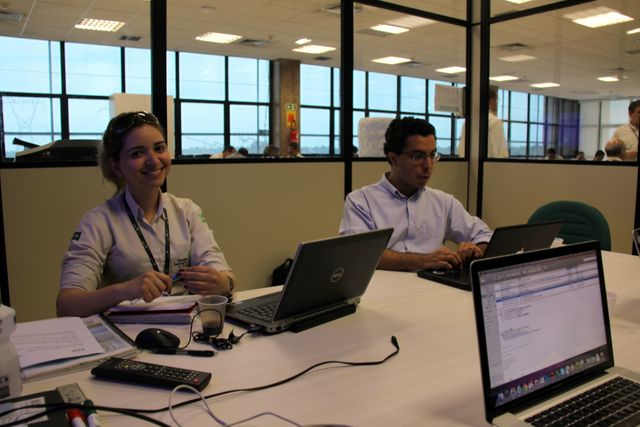
\includegraphics[width=0.6\columnwidth]{figs/jirau/jirau_01}
    \caption{Reunião de abertura.}
    \label{fig:jirau1}
\end{figure}

 \begin{figure}[ht!]
    \centering 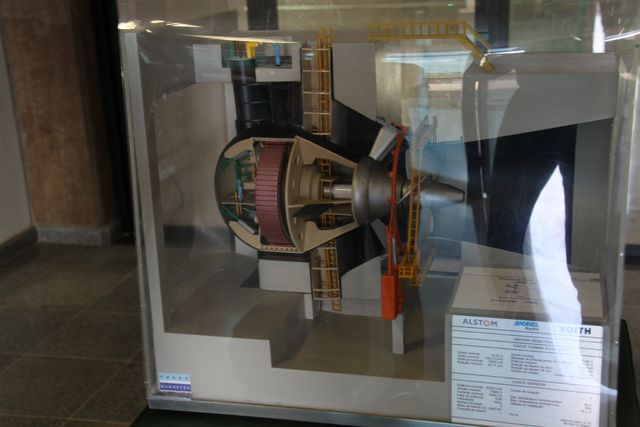
\includegraphics[width=0.6\columnwidth]{figs/jirau/jirau_02}
    \caption{Modelo de turbina da Usina Jirau, observado durante o tour da Usina.}
    \label{fig:jirau2}
\end{figure}

\begin{figure}[ht!]
    \centering 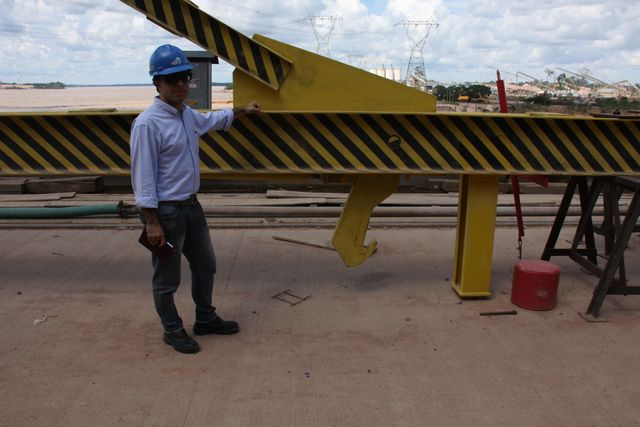
\includegraphics[width=0.6\columnwidth]{figs/jirau/jirau_03}
    \caption{Alessandro Jacoud, no tour pela Usina.}
    \label{fig:jirau3}
\end{figure}

\begin{figure}[ht!]
    \centering 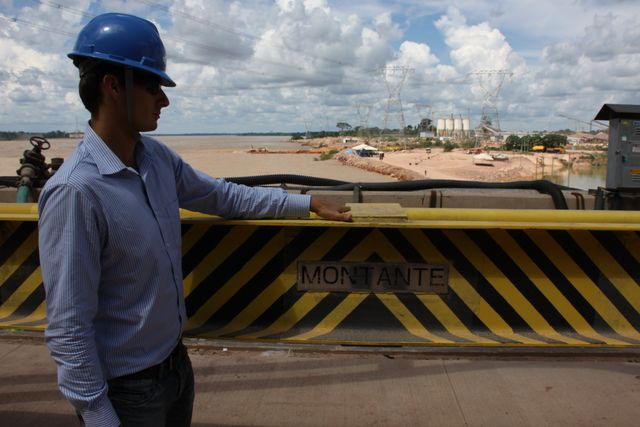
\includegraphics[width=0.6\columnwidth]{figs/jirau/jirau_04}
    \caption{Patrick Paranhos, no tour pela Usina.}
    \label{fig:jirau4}
\end{figure}

\begin{figure}[ht!]
    \centering 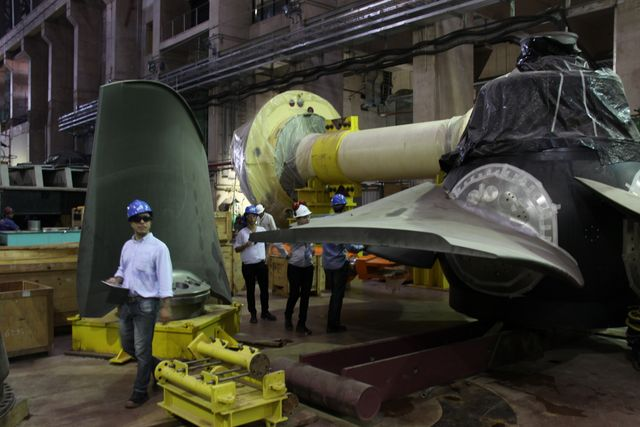
\includegraphics[width=0.6\columnwidth]{figs/jirau/jirau_06}
    \caption{Equipe conhecendo a montagem de turbinas.}
    \label{fig:jirau6}
\end{figure}

\begin{figure}[ht!]
    \centering 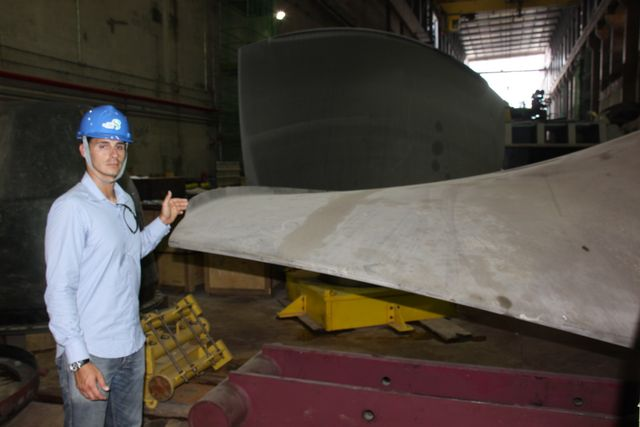
\includegraphics[width=0.6\columnwidth]{figs/jirau/jirau_07}
    \caption{Patrick Paranhos, no tour pela Usina.}
    \label{fig:jirau7}
\end{figure}

\clearpage

Posteriormente a reunião de abertura, o grupo procedeu à análise inicial para
apontar convergências e eventuais contrastes de questões relacionadas à
operação, esclarecendo pontos da solução proposta.  Nessa análise foram
compartilhadas informações de importância relacionadas utilização dos Stoplogs e
de pesquisas já encomendadas pelas ESBR com objetivo de otimizar seu processo de
manutenção de turbinas.
Por fim, foi feita a visita de campo para o acompanhamento da operação de
Stoplog, para que nossa equipe pudesse descrever as etapas do processo a fim de
propor soluções adequadas para contornar as atuais dificuldades no procedimento
de inserção/remoção de Stoplog. Figs.
(\ref{fig:jirau9},\ref{fig:jirau11},\ref{fig:jirau13},\ref{fig:jirau14},\ref{fig:jirau15},\ref{fig:jirau16},\ref{fig:jirau17},\ref{fig:jirau18},\ref{fig:jirau19},\ref{fig:jirau20},\ref{fig:jirau21},\ref{fig:jirau22}).


\begin{figure}[h!]
    \centering 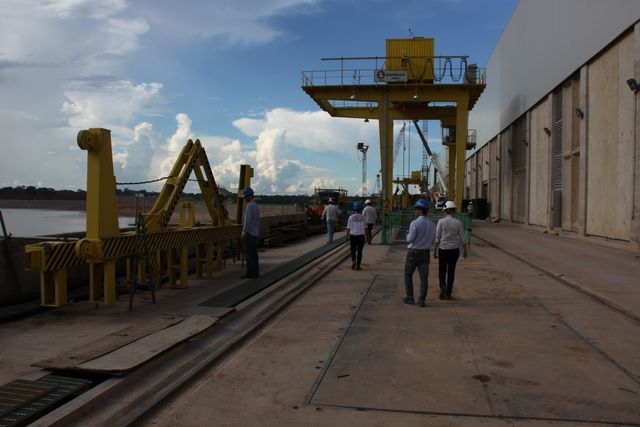
\includegraphics[width=0.6\columnwidth]{figs/jirau/jirau_09}
    \caption{Visita de Campo.}
    \label{fig:jirau9}
\end{figure}

\begin{figure}[h!]
    \centering 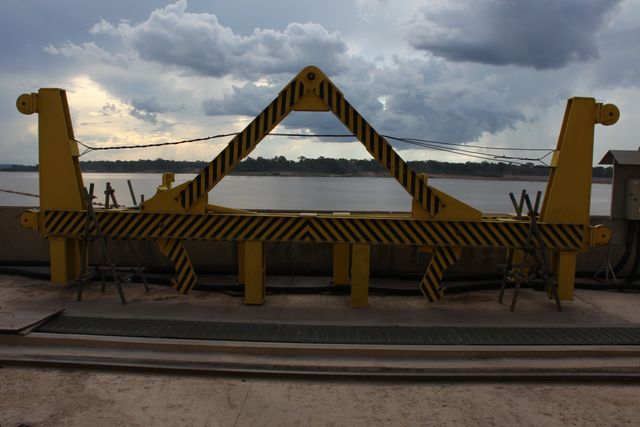
\includegraphics[width=0.6\columnwidth]{figs/jirau/jirau_11}
    \caption{Vista frontal do \emph{Lift beam}.}
    \label{fig:jirau11}
\end{figure}

\begin{figure}[h!]
    \centering 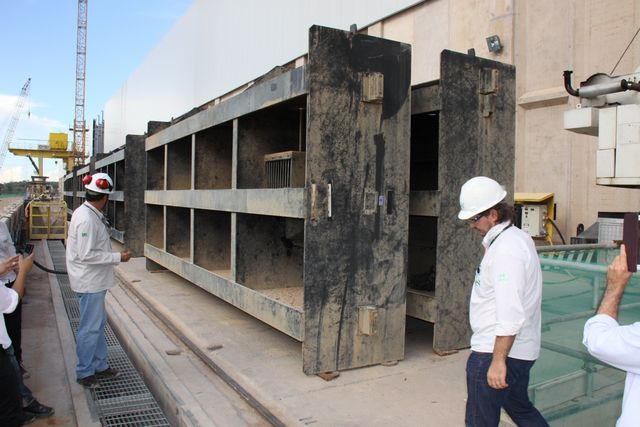
\includegraphics[width=0.6\columnwidth]{figs/jirau/jirau_13}
    \caption{Peça de \emph{Stoplog}.}
    \label{fig:jirau13}
\end{figure}

\begin{figure}[h!]
    \centering 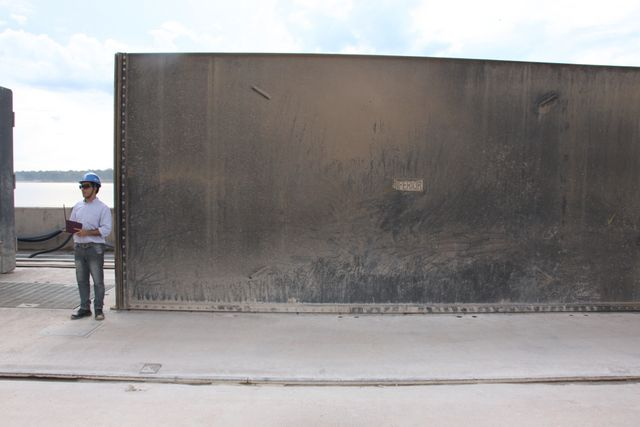
\includegraphics[width=0.6\columnwidth]{figs/jirau/jirau_14}
    \caption{Peça de \emph{Stoplog}.}
    \label{fig:jirau14}
\end{figure}

\begin{figure}[h!]
    \centering 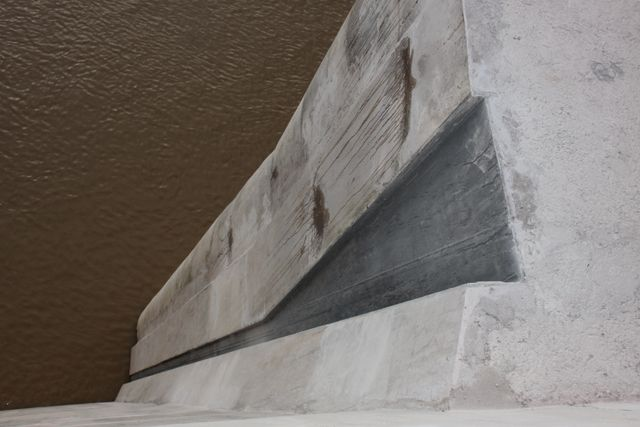
\includegraphics[width=0.6\columnwidth]{figs/jirau/jirau_15}
    \caption{Trilho para as peças de Stoplog.}
    \label{fig:jirau15}
\end{figure}

\begin{figure}[h!]
    \centering 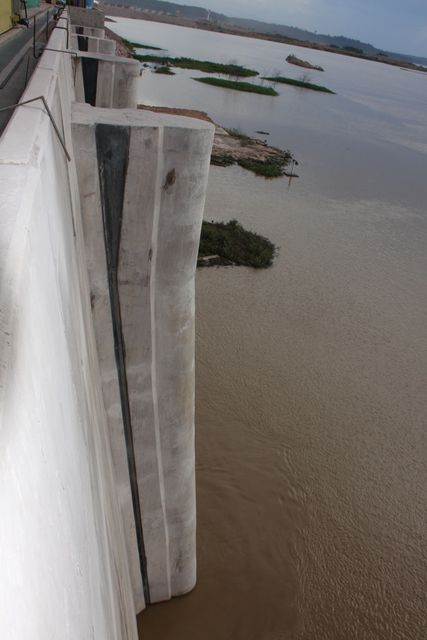
\includegraphics[scale=0.4]{figs/jirau/jirau_16}
    \caption{Trilho para as peças de Stoplog.}
    \label{fig:jirau16}
\end{figure}

\begin{figure}[h!]
    \centering 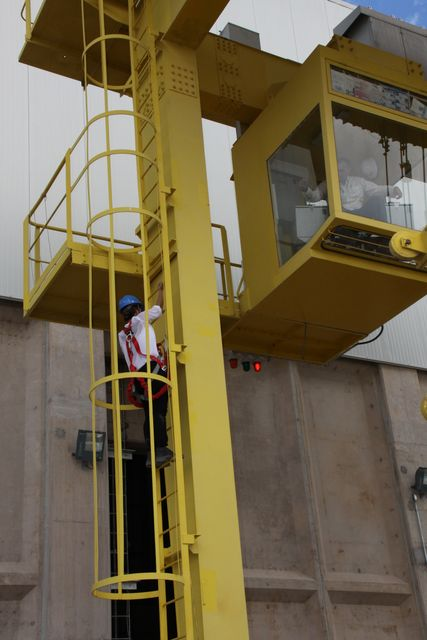
\includegraphics[scale=0.4]{figs/jirau/jirau_17}
    \caption{Parte da análise inclui a observação da operação de \emph{Stoplog} dentro da cabine do operador.}
    \label{fig:jirau17}
\end{figure}

\begin{figure}[h!]
    \centering 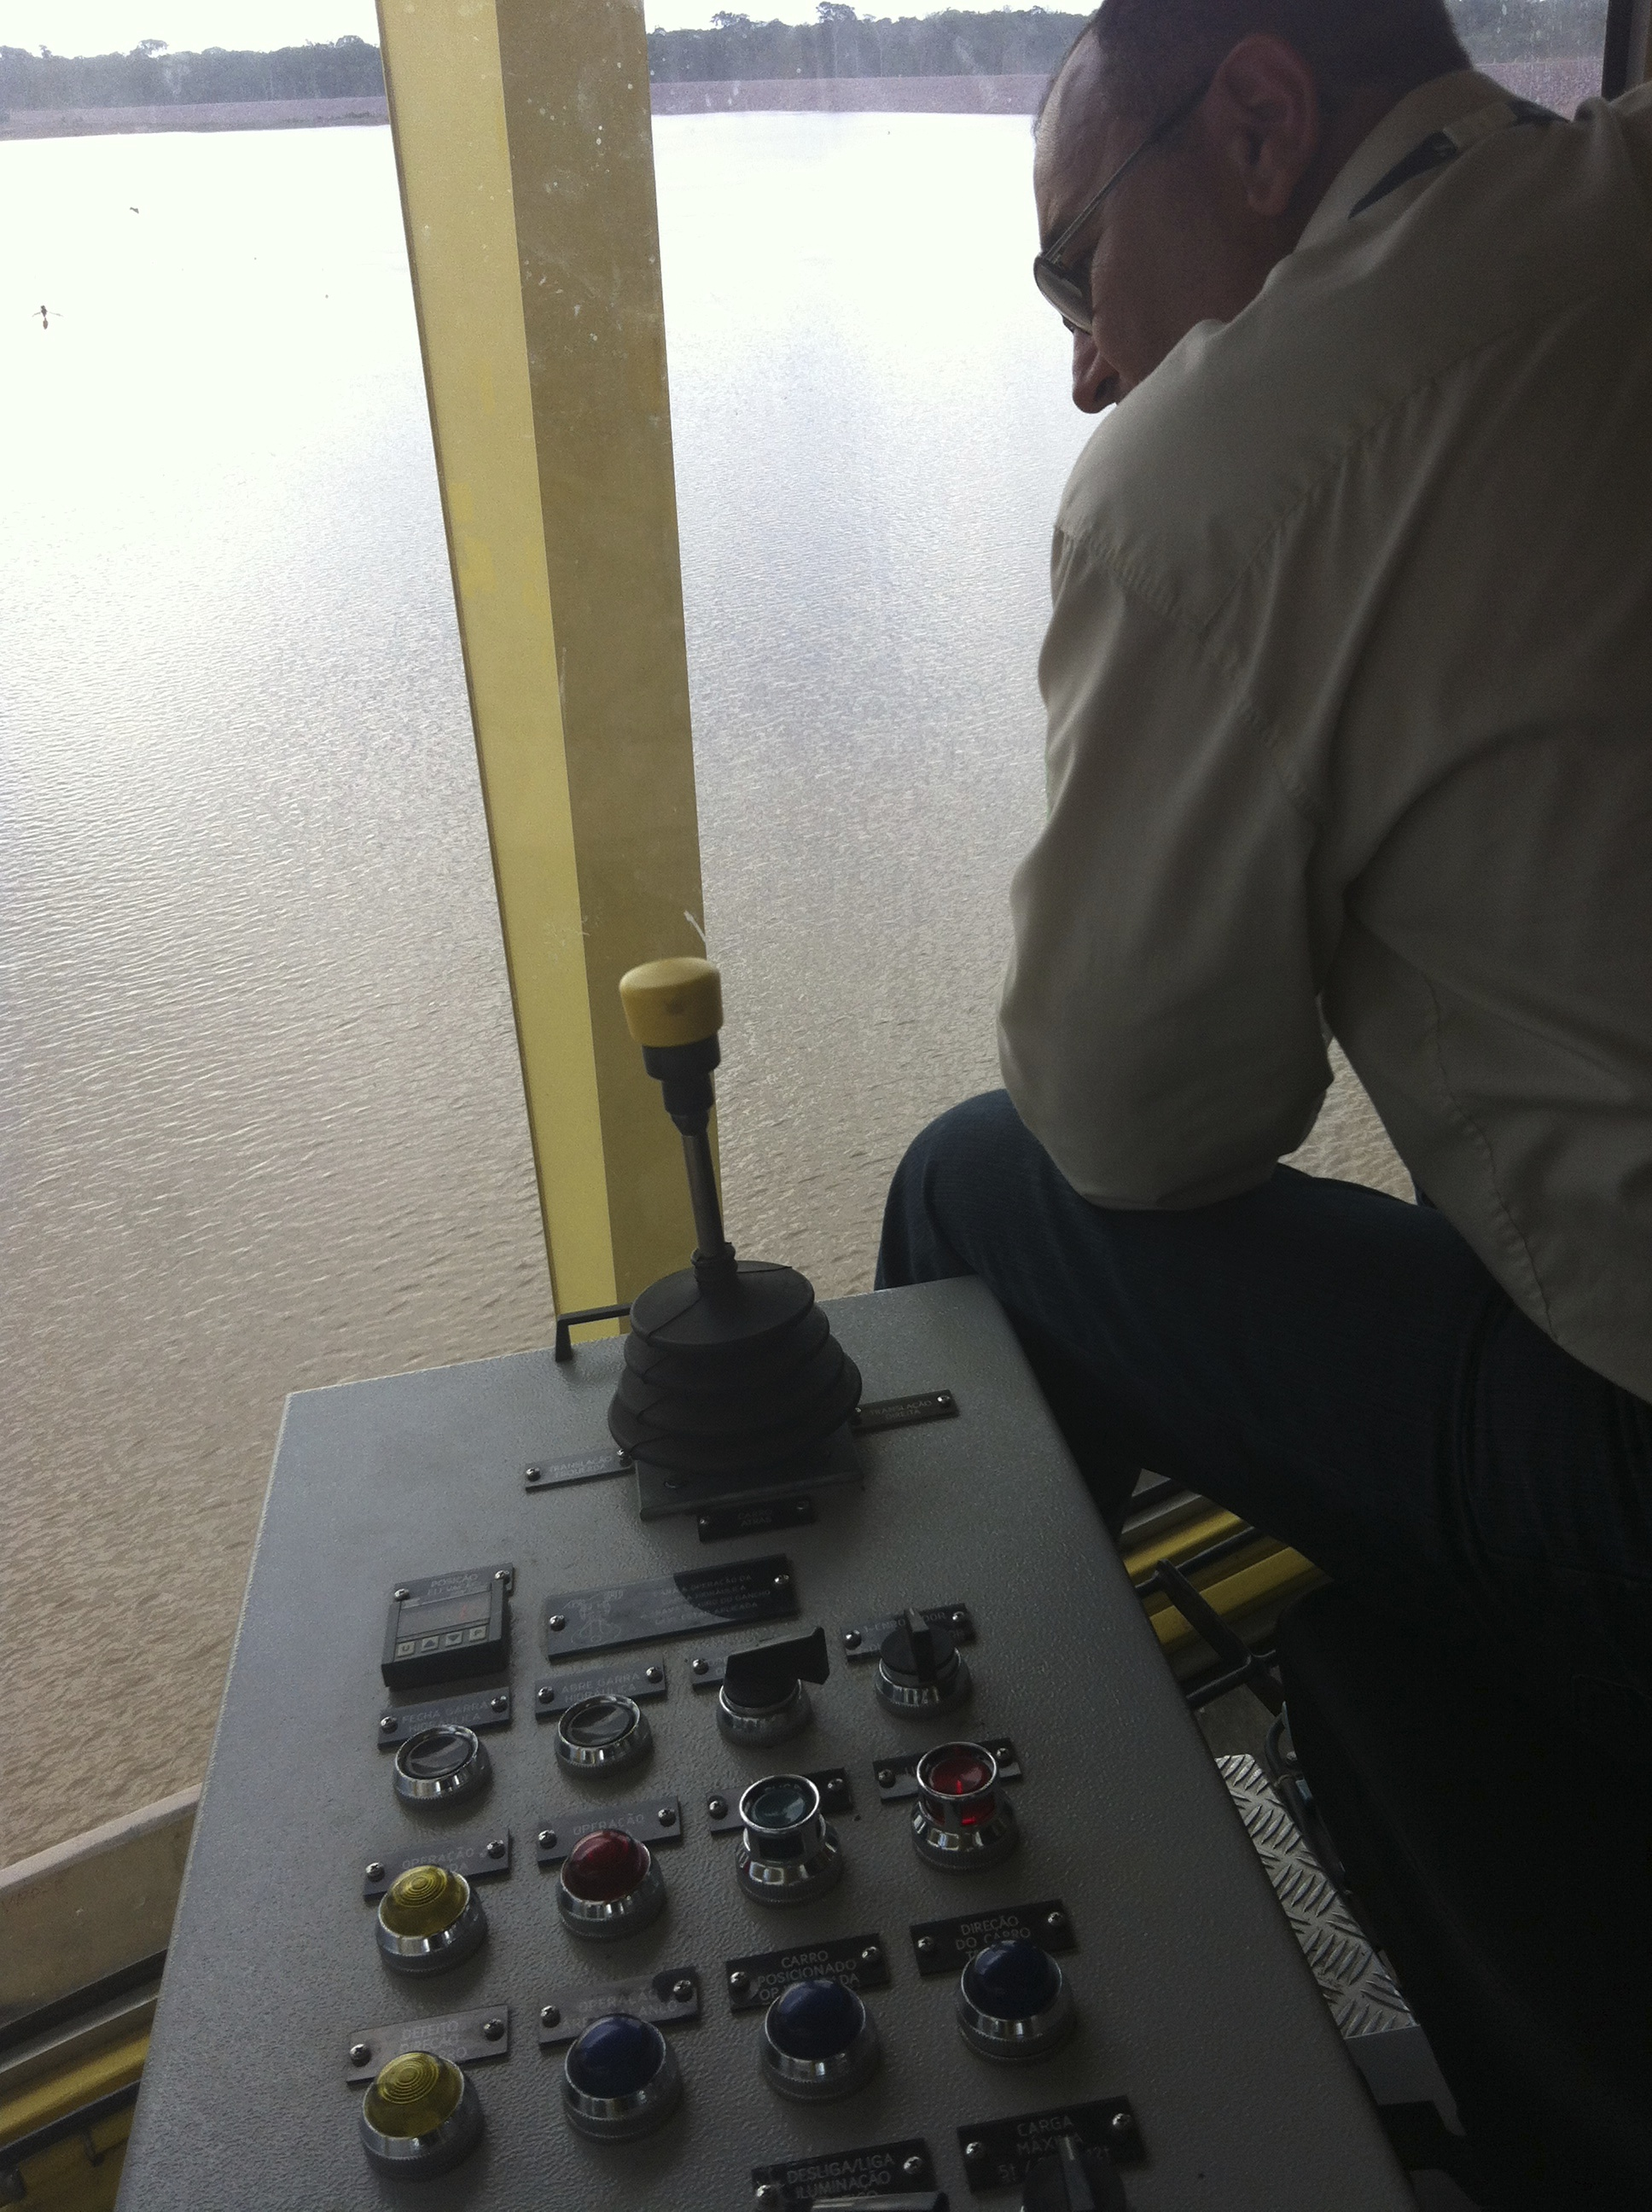
\includegraphics[width=0.5\columnwidth]{figs/jirau/jirau_18}
    \caption{Parte da análise inclui a observação da operação de \emph{Stoplog} dentro da cabine do operador.}
    \label{fig:jirau18}
\end{figure}

\begin{figure}[h!]
    \centering 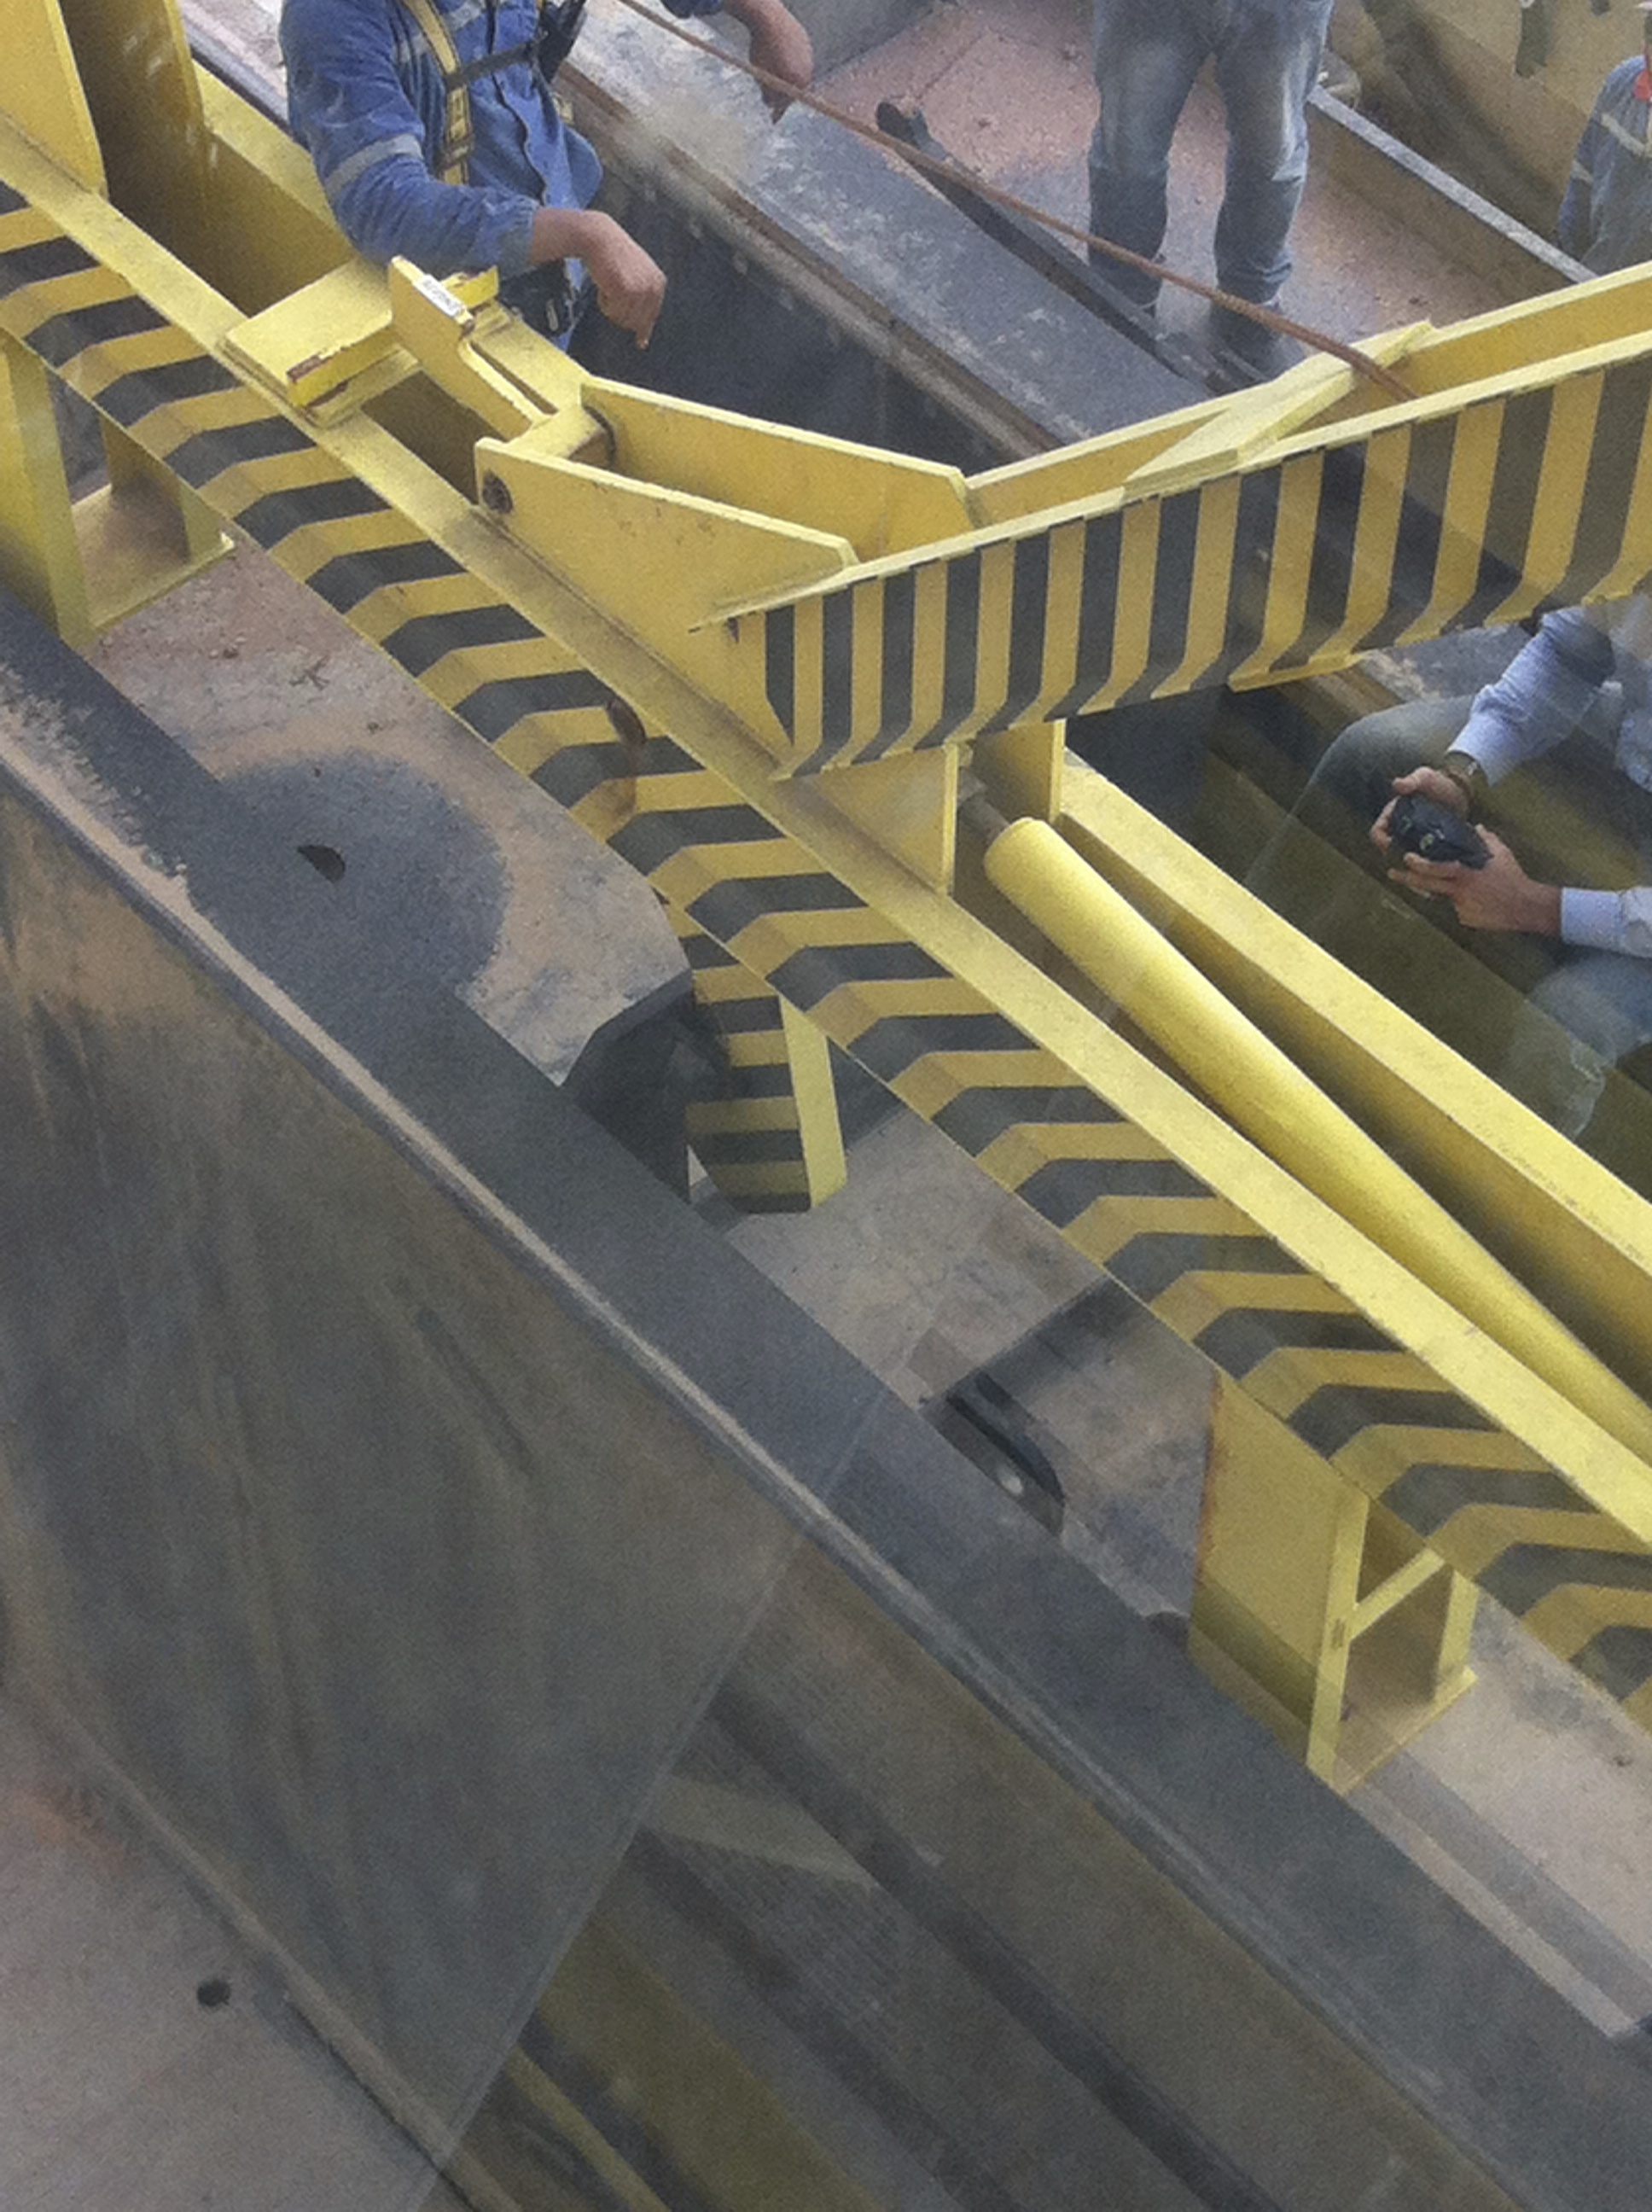
\includegraphics[width=0.5\columnwidth]{figs/jirau/jirau_19}
    \caption{Parte da análise inclui a observação da operação de \emph{Stoplog} dentro da cabine do operador.}
    \label{fig:jirau19}
\end{figure}

\begin{figure}[h!]
    \centering 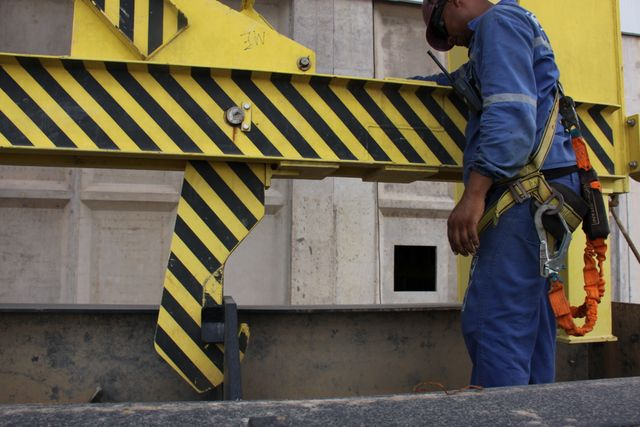
\includegraphics[width=0.6\columnwidth]{figs/jirau/jirau_20}
    \caption{A análise de operação, processo de engate de das garras pescadoras.}
    \label{fig:jirau20}
\end{figure}

\begin{figure}[h!]
    \centering 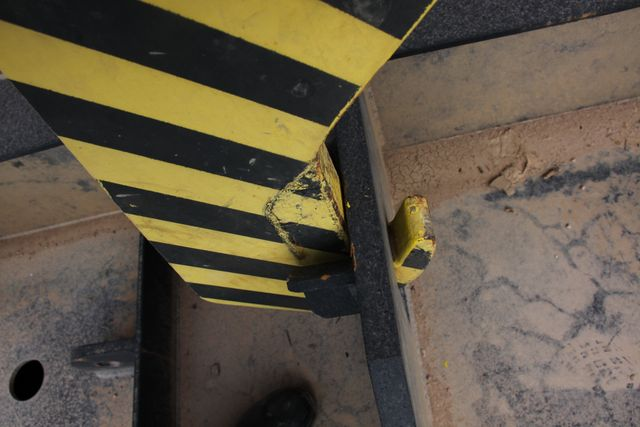
\includegraphics[width=0.6\columnwidth]{figs/jirau/jirau_21}
    \caption{A análise de operação, processo de engate de das garras pescadoras.}
    \label{fig:jirau21}
\end{figure}

\begin{figure}[h!]
    \centering 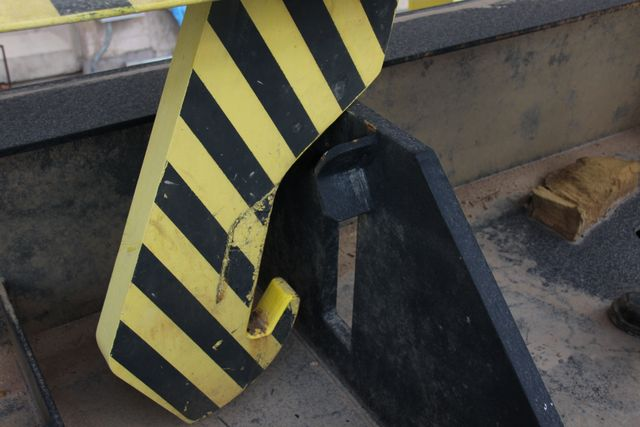
\includegraphics[width=0.6\columnwidth]{figs/jirau/jirau_22}
    \caption{A análise de operação, processo de engate de das garras pescadoras.}
    \label{fig:jirau22}
\end{figure}



\clearpage

Esta seção é subdividida em dois modos de operação padrão: inserção e remoção de
\emph{Stoplogs}. Cada modo de operação padrão possui três modos de operações
excepcionais, realizados em caso de falhas discutidas durante esta seção.

% %******************************************************************************
% % SUBSECTION - Subsection
% %******************************************************************************


\subsection{Operação padrão de inserção}
A operação padrão de inserção consiste: em inserção de \emph{Stoplogs} no Rio
Madeira para o controle de seu fluxo de água, a fim de realizar a manutenção de
turbinas de um sistema de geração de energia elétrica. Esta operação assume as
seguintes \textbf{hipóteses}:
\begin{enumerate}
\item O trilho está livre de obstáculos e sedimentos que poderiam impedir a execução da tarefa.
\label{hip:ins:1}
\item O conjunto \emph{Lifting Beam}/\emph{stoplog} não sofre inclinações e desnivelamento em relação ao trilho, portanto o \emph{stoplog} desliza pelo trilho sem travamento.
\item O desencaixe do conjunto \emph{Lifting Beam}/\emph{stoplog} é realizado com sucesso.
\item O primeiro \emph{stoplog} a ser inserido é posicionado corretamente e veda a base do trilho.
\label{hip:ins:4}
\end{enumerate}

A operação de inserção de \emph{Stoplogs} é composta pelas seguintes
\textbf{etapas}:
\begin{enumerate}
\item Auxiliar de operação manualmente modifica o estado da \emph{chave de operação} para \textbf{Encaixe}.
\item Operador controla o guindaste, o qual desloca o conjunto \emph{Lifting Beam} e \emph{Garras Pescadoras}, até a posição do \emph{Stoplog}, que se encontra em terra, e realiza o encaixe. O encaixe bem sucedido é caracterizado pelo acoplamento correto das duas garras pescadoras com o \emph{Stoplog}. (FIGURA)
\item Auxiliar de operação manualmente modifica o estado da chave de operação para \textbf{Desencaixe}.
\item Operador controla o guindaste, o qual desloca o\emph{Lifting Beam}junto com o \emph{Stoplog}, até os trilhos localizados na barragem, onde os \emph{Stoplogs} deverão ser empilhados.
\item Operador desce o conjunto \emph{Lifting Beam} e \emph{Stoplog} guiado pelo trilho.
\item O desencaixa do conjunto \emph{Lifting Beam}/\emph{Stoplog} é realizado quando o conjunto é impedido de continuar seu curso. Isso ocorre pelo contato do \emph{Stoplog} com o fim da guia ou pelo contato com outro \emph{Stoplog} que já tinha sido posicionado (empilhamento). O desencaixe ocorre, pois, no contato, há perda de tensão no cabo de sustentação do \emph{Lifting Beam} e de forma mecanicamente passiva a garra abre (FIGURA).
\item O procedimento é repetido até os cinco \emph{Stoplogs} estarem empilhados.
\end{enumerate}

Durante todo o procedimento de inserção, o operador pode monitorar o nível de
tensão exercido ao \emph{Lifting Beam} pelo motor elétrico. Um sensor de força
strain gauge é responsável por essa informação, porém há complicações em sua
calibração. Dessa forma, o operador infere o nível de tensão aplicado de acordo
com o ruído sonoro gerado pelo motor.

\subsection{Operação excepcional de inserção 1 - Travamento durante inserção}

Durante a a descida do conjunto  \emph{Lifting Beam}/\emph{Stoplog} pelo operador (etapa 5 da operação padrão de inserção), se assumirmos que o trilho não está livre de obstáculos ou detritos e o \emph{stoplog} começar a se inclinar (falsas as
hipóteses 1 e 2), há a possibilidade de travamento do conjunto com o trilho. Acúmulos de sedimentos e grandes obstáculos
podem impedir a movimentação do \emph{Stoplog}, ou pior, permitir a movimentação
parcial, inclinando a estrutura. Em caso de grande inclinação do conjunto, o
\emph{Stoplog} terá seu movimento impedido e, caso tente-se continuar o processo
de inserção, o \emph{Stoplog} ficará emperrado.

Como o encaixe e desencaixe das \emph{Garras Pescadoras} e o \emph{Stoplog} é
realizado passivamente por meio contato e a tração entre o \emph{Lifiting Beam}
e o \emph{Stoplog}, em caso de travamento do \emph{Stoplog}, haverá perda de tração no cabo e poderá haver
desencaixe parcial ou total. Em caso de desencaixe parcial (apenas uma das
garras), auxiliares mergulhadores são enviados para acoplar o conjunto com cabos
de aço, no local onde ocorreu o desengate. Ao perder o a sustentação de um dos
encaixes, o \emph{Stoplog} descerá inclinado e uma operação para corrigir um
possível travamento deve ser realizada.

Atualmente, quando não há desencaixe, a operação excepcional consiste em um
processo de tentativa e erro, isto é, o operador continuamente ergue e desce o
conjunto \emph{Lifting Beam}/\emph{Stoplog} até a tarefa ser realizada com
sucesso.


\subsection{Operação excepcional de inserção 2 - Falha do desencaixe da garra pescadora}
\label{op:ins:2}

O desencaixe entre a \emph{Garra Pescadora} e o \emph{Stoplog} pode ocorrer
devido a inúmeros fatores. Caso ambas as garras se desencaixe, durante o descida do conjunto \emph{Lifiting Beam}/\emph{Stoplog}, o \emph{Stoplog} se desprenderá do
\emph{Lifiting Beam} e descerá pelo trilho sem controle, podendo acarretar em
sérios danos tanto ao trilho, quanto ao próprio \emph{Stoplog}. Caso ao tocar o fundo ou a superfície de um \emph{Stoplog}, houver um desencaixe mal sucedido de uma das \emph{garras pescadoras}, o \emph{Lifiting Beam} irá levantar o \emph{Stoplog} por apenas um dos olhais e como não há feedback da posição da garra o operador só pode inferir a ocorrência de um desencaixe mal sucedido pela tração do cabo do guindaste. 

Atualmente, em caso de desencaixe
parcial, auxiliares mergulhadores são enviados para mudar a configuração da
\emph{chave de operação} e uma nova tentativa de encaixe pode ser realizada. 

\subsection{Operação excepcional de inserção 3 - Não vedamento devido ao acumulo de detritos na base do trilho}

Uma violação da \textbf{hipótese} \textbf{\ref{hip:ins:1}}, ou seja, existência
de sedimentos ou obstáculos, nesse caso no fundo do rio, pode acarretar em um mau posicionamento do
\emph{stoplog} e/ou má vedação (falha da \textbf{hipótese} \textbf{\ref{hip:ins:4}}).

Atualmente a má vedação só é verificada após a tentativa de drenagem para
inspeção e então é enviado um mergulhador para tirar os detritos. Caso o objeto
seja muito grande haverá um erro de nível, comumente recaindo na \textbf{Operação
excepcional de inserção 3}. 


%_________


\subsection{Operação padrão - Remoção}
A operação padrão de remoção consiste em, basicamente, a operação inversa à da inserção de \emph{Stoplogs}. Esta operação assume as seguintes \textbf{hipóteses}:

\begin{enumerate}
\item Encaixe bem sucedido entre o conjunto \emph{Lifting Beam}/\emph{stoplog}
realizado dentro d'água.
\item Não há acúmulo de sedimentos entre \emph{stoplogs} e entre \emph{stoplog} e base do trilho. Dessa forma, não há diferença extra de pressão hidrostática a ser vencida pelo \emph{Lifting Beam}.
\label{hip:rem:2}
\item O conjunto \emph{Lifting Beam}/\emph{stoplog} se movimenta livremente pelo trilho, sem obstáculos e sedimentos.
\item O conjunto \emph{Lifting Beam}/\emph{stoplog} é removido do trilho e depositado em solo sem sofrer inclinações.  
\item O desencaixe do conjunto \emph{Lifting Beam}/\emph{stoplog} é realizado com sucesso.
\end{enumerate}

A operação de remoção de \emph{Stoplogs} é composta pelas seguintes \textbf{etapas}:
\begin{enumerate}
\item Auxiliar de operação manualmente modifica o estado da \emph{chave de operação} para \textbf{Encaixe}.
\item Operador controla o guindaste, o qual desloca o conjunto \emph{Lifting Beam} pelo trilho até a posição do \emph{Stoplog}, submerso. O encaixe bem sucedido é realizo dentro d'água.
\item O conjunto \emph{Lifting Beam}/\emph{Stoplog} é removido da barragem pelo trilho. 
\item Auxiliar de operação manualmente modifica o estado da chave de operação para \textbf{Desencaixe}.
\item \emph{Stoplog} é depositado em solo.
\item O procedimento é repetido até os cinco \emph{Stoplogs} estarem solo.
\end{enumerate}

\subsection{Operação excepcional de remoção 1 - Falha no encaixe}
\label{op:rem:1}
O encaixe no olhal do \emph{Stoplog} é realizado de forma passiva e sem feedback
quando a operação é realizada submersa. É importante observar que o operador não
recebe nenhum tipo de feedback com relação a encaixe e desencaixe da garra
pescadora. Como a operação é realizada debaixo d'aguá, sem visibilidade, o
processo de encaixe no \emph{Stoplogs} se torna uma longa série de tentativas e
erros, na qual o \emph{Lifting Beam} é suspenso e submerso inúmeras vezes.

Um encaixe mal sucedido durante a etapa 1 (a hipótese 1 não satisfeita) pode ser
decorrente de uma tentativa de encaixe com o \emph{Lifiting Beam} inclinado ou
por detritos presentes no olhal do \emph{Stoplog} ou em sua superfície. Um
encaixe mal sucedido pode acarretar em um desencaixe durante o percurso ou um
encaixe parcial, ocasionando na queda ou travamento do \emph{Stoplog}
(necessitando a realização da \textbf{Operação excepcional de remoção 2}).

Em caso de desencaixe parcial (apenas uma das garras), auxiliares mergulhadores
são enviados para alterar a posição da \emph{Chave de Operação}, para a
realização do desencaixe das \emph{Garras Pescadoras}. Quando o desencaixe
parcial não é percebido em tempo hábil, devido a ausência de feedback (operação
submersa), o \emph{Stoplog} realizará, mais uma vez, apenas movimentação parcial
e um possível travamento (\textbf{Operação excepcional de remoção 2}).

Caso não ocorra nenhum encaixe, é realizada múltiplas tentativas até um encaixe
completo. Entretanto, se não houver sucesso, mergulhadores são enviados para a
inspeção do olhal e da superfície do \emph{Stoplog} a procura de detritos
obstruindo o encaixe.

\subsection{Operação excepcional de remoção 2 - Travamento durante remoção}
\label{op:rem:2}

Caso o conjunto \emph{Lifiting Beam/Stoplog} não possa se mover livremente pelo trilho (hipótese 3 não satisfeita), o conjunto poderá começar a se inclinar e, assim, ocasionar um possível travamento do sistema. O único feedback presente nesse tipo de erro é a tração no cabo do guindaste, o que significa que uma vez que a tração se altere o \emph{Stoplog} já não está se movendo livremente, não sendo possível realizar uma operação preventiva e apenas uma ação corretiva para o travamento durante a inserção.

\subsection{Operação excepcional de remoção 3 - Acúmulo de sedimentos no fundo}
\label{op:rem:3}
Uma vez que a inserção é realizada com sucesso, mantendo então a \textbf{hipótese}
\textbf{\ref{hip:ins:4}}, pode-se ocorrer um posterior acúmulo de sedimentos na
base, ou seja, uma violação da \textbf{hipótese} \textbf{\ref{hip:rem:2}}.

Os sedimentos acumulados no vão inferior (vide figura \ref{fig:op:rem:3_1}) do
\emph{stoplog} em contato com o solo ocasiona um efeito efeito ventosa. Eles
formam uma barreira que forma uma contenção à pressão hidrostática da água (vide
figura \ref{fig:op:rem:3_2})  eliminando a força devido ao princípio de
arquimedes.

As medidas tomadas atualmente consistem apenas em força bruta. Puxa-se o
\emph{stoplog} com um guindaste com força suficiente para vencer a pressão da
coluna d'água, o que comumente acarreta em danos ao próprio \emph{stoplog} e aos
equipamentos envolvidos.

\begin{figure}[h!]
    \centering
    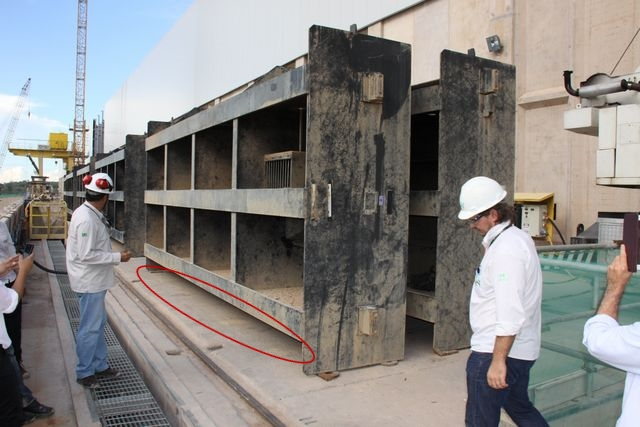
\includegraphics[width=0.6\columnwidth]{figs/modos/op_rem_3/op_rem_3_1.jpg}
    \caption{Local onde ocorre o acúmulo de sedimentos no fundo.}
    \label{fig:op:rem:3_1}
\end{figure}


\begin{figure}[h!]
    \centering
    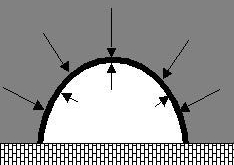
\includegraphics[width=0.6\columnwidth]{figs/modos/op_rem_3/op_rem_3_2.jpg}
    \caption{Pressão interna se torna muito menor que a externa devido ao
    isolamento causado pelos sedimentos.}
    \label{fig:op:rem:3_2}
\end{figure}


